% Created 2013-12-20 金 04:52
\documentclass[12pt]{jsarticle}
\usepackage[dvipdfmx]{graphicx}
\usepackage{comment}
%\usepackage{setspace}
%%\date{\today}
%\title{}
\textheight = 25truecm
\textwidth = 18truecm
\topmargin = -1.5truecm
\oddsidemargin = -1truecm
\evensidemargin = -1truecm
\marginparwidth = -1truecm
\def\theenumii{\Alph{enumii}}
\def\theenumiii{\alph{enumiii}}
\def\labelenumi{(\theenumi)}
\def\labelenumiii{(\theenumiii)}
%\setstretch{0.9}
\begin{document}

%\maketitle
%\tableofcontents

\begin{center}
%%%%%%%%%%%%%%%%%%%%%%%%%%%%%%%%%%%%%%%
%%%タイトル                         %%%
%%%%%%%%%%%%%%%%%%%%%%%%%%%%%%%%%%%%%%%
{\LARGE 共有メモリを用いたデータの受け渡しの確認}
\end{center}

\begin{flushright}
  2014/9/17\\
  藤田将輝
\end{flushright}
%%%%%%%%%%%%%%%%%%1章%%%%%%%%%%%%%%%%%%%
\section{はじめに}

共有メモリを用いてのデータの受け渡しが成功していることを確認した.
本資料ではNICドライバへの割り込み挿入法の概要,使用する共有メモリの先頭アドレス,および共有メモリを用いたデータ受け渡しの確認
について述べる.


\section{NICドライバへの割り込み挿入手法の概要}

Mintを用いて,割り込み元OSから割り込み先OSのNICドライバへ割り込みを挿入する流れを図1に示し,以下で説明する.
\begin{enumerate}
\item 割り込み情報の指定

プログラマが割り込みジェネレータを用いて割り込み情報を指定する.
\item 割り込み情報の通知

割り込みジェネレータから割り込み元OSのデバッグ支援機構へ割り込み情報を通知する.
\item パケットの生成

割り込み元OSのデバッグ支援機構がパケットを生成する.
\item 受信バッファへのパケットの格納

割り込み元OSのデバッグ支援機構が受信バッファへパケットを格納する.
\item 受信バッファ状態の更新

割り込み元OSのデバッグ支援機構が受信バッファ状態を受信済み状態へ更新する.
\item 割り込み発生要求

割り込み情報をもとに,割り込み元OSのデバッグ支援機構からコア0へ割り込み発生要求を行う.
\item IPI の送信

割り込み元OSが保持するコア0から割り込み先OSが保持するコア1へIPIを送信する.
\item 割り込み処理の開始

割り込み先OSが割り込み処理を開始する.この際,割り込み先OSが割り込みベクタ番号に対応した割り込みハンドラを実行する.
\item 受信バッファの特定

受信ディスクリプタが保持する受信バッファ状態を割り込み先OSのNICドライバが参照する.これにより,パケットが格納されている受信バッファを特定する.
\item ソケットバッファへのパケットの格納

受信バッファからソケットバッファへ割り込み先OSのNICドライバがパケットを格納する.

\begin{figure}[t]
\begin{center}
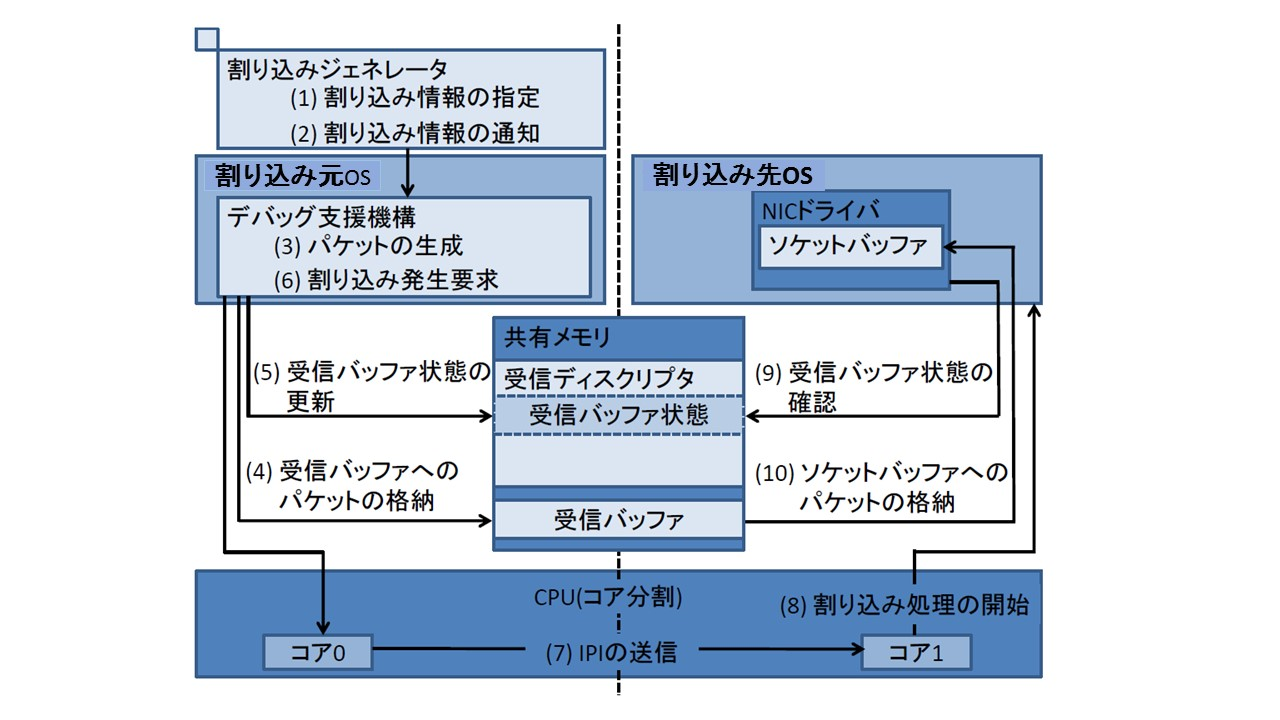
\includegraphics[height=8.0cm]{./fig1.jpg}          
\caption{NICドライバへの割り込み挿入の流れ}
\label{fig:up}
\end{center}
\end{figure}



\end{enumerate}
\section{使用する共有メモリ領域の先頭アドレス}
Mintには共有メモリが用意されている.
この様子を図2に示し,以下で説明する.
具体的には0x1000000~0x2000000が共有メモリとして用意されている.
共有メモリ領域の先頭アドレスにはMintのコア管理表のための領域が確保されている.
NICドライバへのデータを格納する領域を確保するため,コア管理表が使用している領域の終端アドレスを確認する必要がある.
このため,コア管理表を作成しているプログラム「mint\_cpumap.c」の中にある,共有メモリを参照している関数の
一部をシステムコールとして新たに作成し,調査した.
これにより,0x1000018までを使用していることが分かった.
このため,本実験では,0x1000019以降を使用する.
なお,実際にデバッグ支援機構として利用する領域については別途検討する.


\begin{figure}[t]
\begin{center}
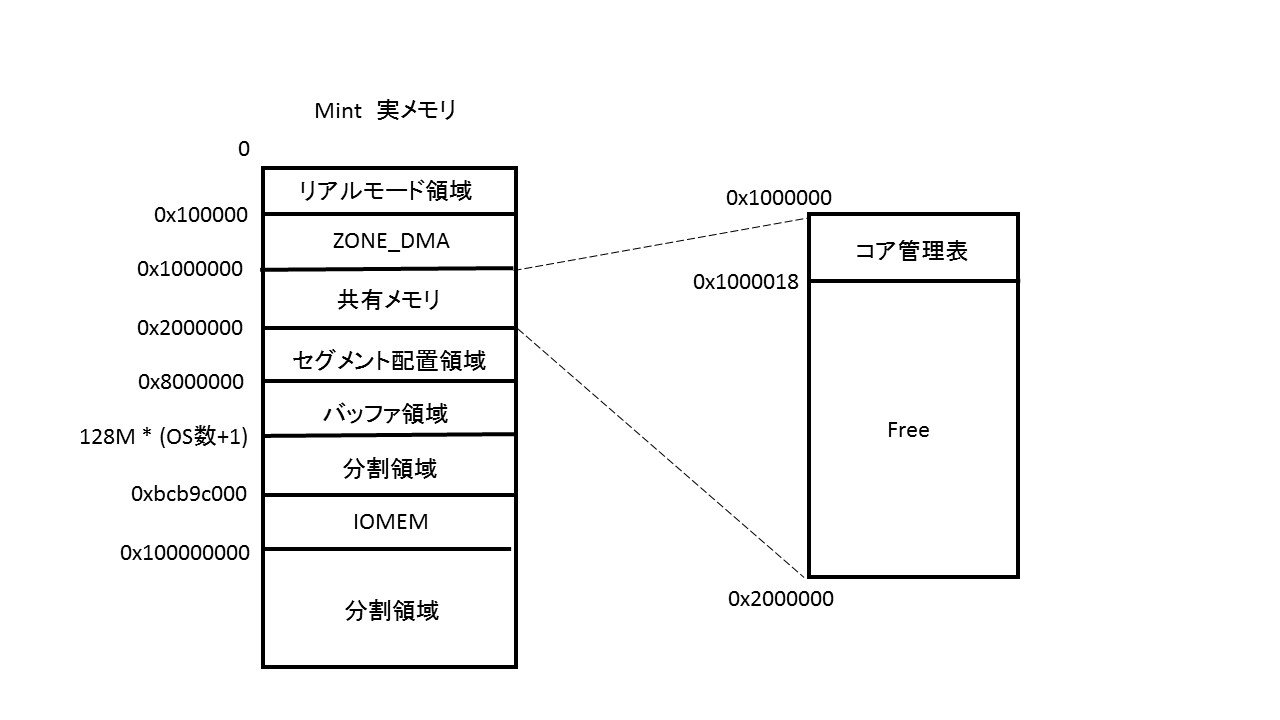
\includegraphics[height=8.0cm]{./fig2.jpg}          
\caption{Mint共有メモリ}
\label{fig:up}
\end{center}
\end{figure}


\section{共有メモリを用いたデータ受け渡しの確認}
共有メモリを使用し,OSノード間のデータの受け渡しの確認をするため,簡単な例として,配列に
文字列を格納し,データの受け渡しを確認した.
具体的には割り込み先OSで「fujita」という文字列を格納した配列を0x1000020に格納し,
割り込み元OSで0x1000020から配列に文字列を複写し,これを確認した.
どちらもシステムコールにより実現した.
0x1000020は仮の使用アドレスとする.
以下に流れを示す.
\begin{enumerate}
\item 割り込み元OSでシステムコールを発行する.
\item システムコールにより,「fujita」という文字列が格納された配列から文字列を共有メモリの0x1000020に格納する.
\item 割り込み先OSでシステムコールを発行する.
\item システムコールにより,共有メモリの0x1000020から文字列を配列に格納し,標準出力に表示する.
\end{enumerate}

\section{おわりに}
本資料ではNICドライバへ割り込みを挿入する際のデータの受け渡しについて記述した.
割り込み元OSでデータを共有メモリ領域に格納し,割り込み先OSで共有メモリに格納されたデータを取得できることを確認した.
今後は,使用する共有メモリ領域のサイズ,格納するデータの構造を調査し,本機構における共有メモリ領域の利用法について検討し,実装する.


\end{document}
